در شکل زیر ۵ عدد میخ مشاهده می‌کنیم که با تعدادی کش به هم متصل شده‌اند. به چند طریق می‌توان ۵ گش انتخاب کرد به نحوی که هر میخ دقیقا به دو کش انتخاب شده وصل باشد؟
\begin{center}
  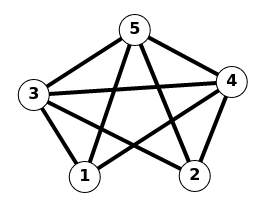
\includegraphics[width=.5\linewidth]{CombinatorialAnalysis/Problems/16/E9_4_1.png}
\end{center}